\question \textbf{Life of Alex} \newline
Alex is enjoying college life. She spends a day either studying, 
partying, or looking for housing for the next year. If she is studying, 
the chances of her studying the next day are 30\%, the chances of her 
partying the next day are 50\%, and the chances of her looking for 
housing the next day are 20\%. If she is partying, the chances of her 
partying the next day are 10\%, the chances of her studying the next 
day are 60\%, and the chances of her looking for housing the next day 
are 30\%. If she is looking for housing, the chances of her looking 
for housing the next day are 50\%, the chances of her partying the 
next day are 30\% and the chances of her studying the next day are 20\%.

\begin{enumerate}[label=(\alph*)]
\item Draw a Markov chain to visualize Alex’s life.
\begin{solution}[5cm]
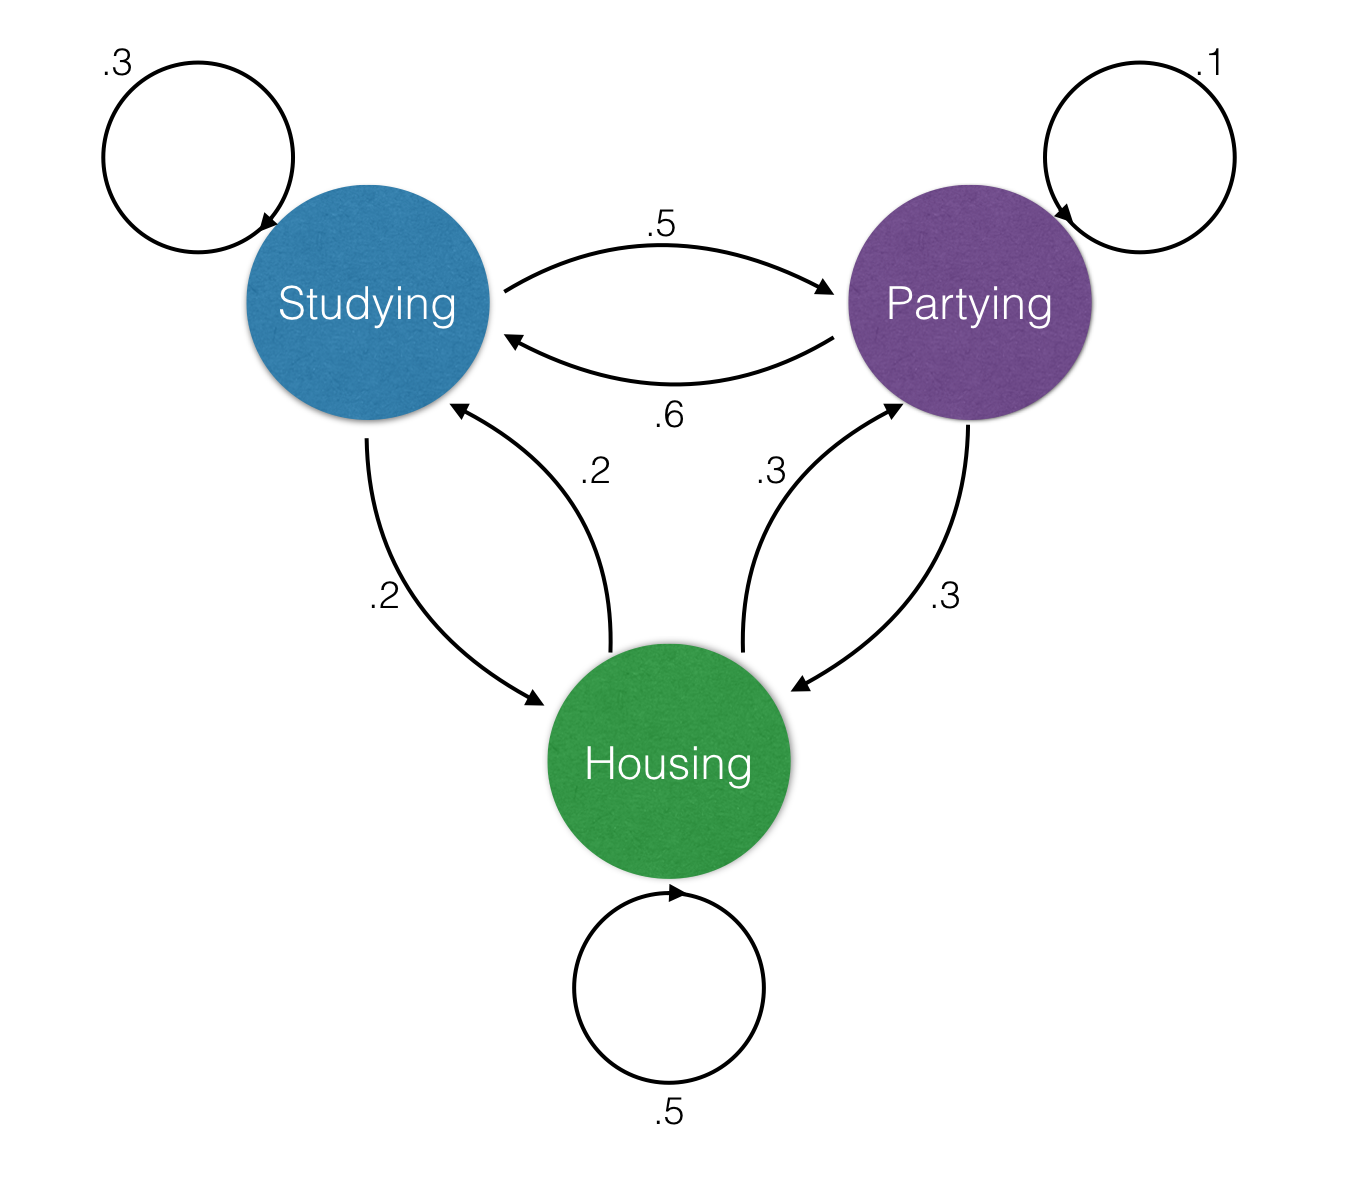
\includegraphics[width=8cm]{life_of_alex.jpg}
\end{solution}

\item Write out a matrix to represent this Markov chain.
\begin{solution}[3cm]
\[\begin{bmatrix}
.3 & .5 & .2 \\
.6 & .1 & .3\\
.2 & .3 & .5
\end{bmatrix}
\]
\end{solution}

\item If Alex studies on Monday, what is the chance that she is 
partying on Friday? (Don't do the math, just write out the expression 
that you would use to find it.)
\begin{solution}
If $P$ is the matrix above, then it is $[1, 0, 0] \cdot P^4$
\end{solution}
\clearpage

\item What percentage of her time should Alex expect to use looking 
for housing?
\begin{solution}[5cm]
Solve the following system of equations: (first step equations)
\begin{equation}
\begin{split}
S &= .3S + .6P + .2H \\ \nonumber
P &= .5S + .1P + .3H \\
H &= .2S + .3P + .5H \\
S + P + H &= 1
\end{split}
\end{equation}
\end{solution}

\item If Alex parties on Monday, what is the chance of Alex partying 
again before studying?
\begin{solution}[3cm]
Set up the following equations:
\begin{equation}
\begin{split}
H1 &= 0 \\ \nonumber
H2 &= .6(H1) + .1(1) + .3(H3) \\
H3 &= .2(H1) + .3(1) + .5(H3)
\end{split}
\end{equation}
Solving for $H2$, we get 0.28
\end{solution}

\end{enumerate}